% !TEX TS-program = pdflatex
% !TEX encoding = UTF-8 Unicode

% This is a simple template for a LaTeX document using the "article" class.
% See "book", "report", "letter" for other types of document.

\documentclass[12pt]{article} % use larger type; default would be 10pt

\usepackage[utf8]{inputenc} % set input encoding (not needed with XeLaTeX)

%%% Examples of Article customizations
% These packages are optional, depending whether you want the features they provide.
% See the LaTeX Companion or other references for full information.

%%% PAGE DIMENSIONS
\usepackage{geometry} % to change the page dimensions
\geometry{letterpaper} % or letterpaper (US) or a5paper or....
% \geometry{margin=2in} % for example, change the margins to 2 inches all round
% \geometry{landscape} % set up the page for landscape
%   read geometry.pdf for detailed page layout information

\usepackage{graphicx} % support the \includegraphics command and options

% \usepackage[parfill]{parskip} % Activate to begin paragraphs with an empty line rather than an indent

%%% PACKAGES
\usepackage{amsmath} %for making equations
\usepackage{amssymb}
\usepackage{bbm}
\usepackage{subfig}
\usepackage{mwe}
\usepackage{graphicx}
\graphicspath{{C:/Users/Gabrielle/Desktop/Figures/}}
\usepackage{epstopdf}
\usepackage{grffile}
\usepackage{indentfirst}
\usepackage{tikz}
\usepackage{tikzscale}
\usepackage{pgfplots}
\usepackage{booktabs} % for much better looking tables
\usepackage{array} % for better arrays (eg matrices) in maths
\usepackage{paralist} % very flexible & customisable lists (eg. enumerate/itemize, etc.)
\usepackage{verbatim} % adds environment for commenting out blocks of text & for better verbatim
\usepackage{subfig} % make it possible to include more than one captioned figure/table in a single float
% These packages are all incorporated in the memoir class to one degree or another...

%%% HEADERS & FOOTERS
\usepackage{fancyhdr} % This should be set AFTER setting up the page geometry
\pagestyle{fancy} % options: empty , plain , fancy
\renewcommand{\headrulewidth}{0pt} % customise the layout...
\lhead{}\chead{}\rhead{}
\lfoot{}\cfoot{\thepage}\rfoot{}

%%% SECTION TITLE APPEARANCE
\usepackage{sectsty}
\allsectionsfont{\sffamily\mdseries\upshape} % (See the fntguide.pdf for font help)
% (This matches ConTeXt defaults)

%%% ToC (table of contents) APPEARANCE
\usepackage[nottoc,notlof,notlot]{tocbibind} % Put the bibliography in the ToC
\usepackage[titles,subfigure]{tocloft} % Alter the style of the Table of Contents
\renewcommand{\cftsecfont}{\rmfamily\mdseries\upshape}
\renewcommand{\cftsecpagefont}{\rmfamily\mdseries\upshape} % No bold!

%%% END Article customizations

%%% The "real" document content comes below...

\title{MS Project: Map Simulations (Draft)}
\author{Gabrielle Cole}
\date{} % Activate to display a given date or no date (if empty),
         % otherwise the current date is printed 

\begin{document}
\maketitle
\tableofcontents

\section{Abstract}

In this paper we present a simulation in which the signal to noise measurements are obtained for galaxy clusters at various redshifts and masses. We begin with an introduction to the data which this simulation attempts to model and an overview of a variety of related topics necessary to understand the results later presented. In section 2, an explanation of the various techniques used as well as simplifying assumptions made is given. Finally, in section 3, results are presented and in the subsequent section, discussed. 
 

\section{Introduction}

The South Pole telescope, which conducts large area milimeter and sub-milimeter surveys of the anisotropies (tiny tempeture fluxuations) caused by the cosmic microwave background, has produced data that in conjunction with the Sunyaev-Zel'dovich effect can be used to detect galaxy clusters. These clusters are of great interest for a number of reasons: (1) Galaxy clusters are some of the largest gravitationally bound structures in our known universe and thus serve as markers of large scale matter density giving us insight into the current overall composition of our universe. (2.) Galaxy clusters can also tell us quite a bit about the early history of the universe as their formation is generally agreed to be due in large part to the localized matter density fluctuations caused by the early inflationary epoch. It was during this inflationary epoch that universe underwent a rapid expansion that seeded much of the structure (in the form of massive galaxy clusters) we observe today. Later, as a result of recombination (when most electrons became bound to ions) the lenght scale on which graviational collapse could occur dropped allowing for those seeds of structure (created during the inflationary epoch) to become the large scale stuctures, namely galaxy clusters, that we observe today (3.) Galaxy clusters contain much of the matter of the universe and thus provide a rich laboratory in which to examine the universe. For instance, in galaxy clusters that we find stars, plasma, black holes, dark matter, and molecular gases. We also witness blazars, supernova, and quasars in galaxies which are located within clusters. (4.) Finally, galaxy clusters are of great interest because they provide a relatively rich array of observational data. That is to say that clusters produce detectable signals across a wide range of the electromagnetic spectrum and are thus natural objects for observation. All of this taken together then, the case for clusters as cosmological probes is compelling. 

Briefly, the actual composition of clusters should be noted. On average clusters are composed primarily of Dark Matter (90\% by mass), of which little is concretely known. Dark Matter's existance is primarily inferred from the inablity of known matter to explain observed graviational effects on visible matter.  In the middle the intracluster medium or ICM composes ~9\%, by mass, of a cluster. The ICM can be colloquially referred to as hot gas, in fact the ICM is extremely hot gas, or plasma, (around $10^{7} - 10^{8}$ K) which exhibits strong X-ray emissions. These emissions can be used for cluster dection and as a check on dectections carried out using the Sunyaev-Zel'dovich explained later in this introduction. Surprisingly, the smallest component of galaxy clusters is the galaxies themselves (less than 1\% by mass). A typical galaxy cluster may contain upwards of thousands of indiviual galaxies which themselves are composed of stars, more gas and dust. 

Clusters are not a homogenous group, rather they have a diverse properties and can therefore be divided into subclasses. For example, in rich clusters, (clusters with hundreds to thousands of galaxies), elliptical galaxies tend to gather near the center of the cluster whereas spiral galaxies are normally found near the periphery. However, poor clusters, clusters with only a few galaxies, do not exhibit this pattern and in general have a more irregular morphology as a result of being less able to hold their member galaxies in toe. 

The diversity of clusters themselves suggest that within a single cluster the observed physics can vary as one looks at differing locations within that single cluster. And in fact it is the case that each section of a galaxy cluster, moving from its center outward, exhibits different types of physics. In general our ablity to decipher the type of interactions occuring in clusters and to detect their existance in the first place is highly dependent on the cluster's density (specifically, the ICM). However, cluster density (and therefore our ablity to detect and characterize interactions) tends to fall off as one moves outward from the center of the cluster. Therefore, it is unsurprising that much of the physics occurring at the outskirts of galaxy clusters remains unknown as the low signal to noise ratios have limited the analysis that could be performed. However, recently, because of the proliferation of overlapping data sets as well as advances in detection equipment, the ability to examine the physics of these outer edges is becoming increasingly feasible. Nevertheless, in order to make headway, a model is needed to bound expectations on the data eventually obtained. That is to say, we must create and analyze a realistic simulation of the expected data to both provide reasonable expectations on the anticipated signal to noise ratio before a measurment is taken  and to eventually be used to check against the obtained data after the measurment is taken. 

Broadly, therefore, the simulation must at least include the following three components: (1.) The isotropic CMB (cosmic microwave background) thermal radiation leftover from the early universe. (2.) Cluster profiles: puesdo-randomly distributed over the field of sight  (cluster mass is correlated to redshift, and therefore purely random distribution would be inaccurate) and finally (3.) Noise: random Gaussian background noise created by the detection device (the telescope)  Each of the three elements of the simulation deserve a brief introduction which we now give: 

We begin, naturally, with a brief introduction to the CMB as it relates to this work.  The cosmic microwave background is acutally relic radiation left over from the Big Bang, simply the CMB radiation is composed low energy (and very old) photons. The radiation caused by these photons is extremely close to perfect blackbody radiation, with a spectrum characterized by a single temperature (2.7 K). For completness, we further explain what we mean by perfect blackbody radiation: All objects spontaneously emit thermal radiation (usually in the infrared where it cannot be seen). This radiation is emitted over a range of frequencies and is correlated to the absolute temperature of the object. A blackbody is an object which absorbs all incident radiation regardless of frequency. Both objects in thermodynamic equilibrium and blackbodies at constant and uniform temperature emit blackbody radiation. The wonderful thing about this type of radiation is that its spectrum depends solely on the object's temperature. This is simply to say that the photons of the CMB radiation can be quite percisely characterized and represent a highly isotropic (or uniform) radiation field. For example, the peak brightness of the CMB radiation is around $3.7 \times 10^{-18} \frac{W}{m^{2} \cdot Hz \cdot sr}$  at a frequency of 160 GHz, its photon density around 4 $\times 10^{8}$ photons $\cdot m^{-3}$, and it's mass density around 5$\times 10^{-31}$ kg $\cdot m^{-3}$. Curiously, this density is much less than the critical density, $\rho_c$, necessary to prevent the universe from either slowing in expansion and eventually collapsing or expanding forever. 

Again we must take a slight detour to explain what we mean by the critical density, $\rho_c$. Typically, the matter density parameter, $\Omega$, is defined as the ratio of the actual density of the universe to the critical density: $\frac{\rho}{\rho_c}$. So if the actual density, $\rho$ is greater than $\rho_c$, then $\Omega$ is greater than unity and the eventual fate of the universe will be slowed expansion and eventual collapse. In this case the geometry of the universe is closed, much like a beach ball, if you are traveling for long enough any any direction along its surface you will end up back where you began. Conversely, if the actual density, $\rho$ is less than $\rho_c$, then $\Omega$ is less than unity and the eventual fate of the universe will be continued expansion. In this case the geometry of the universe is hyperbolic. If however the actual density, $\rho$ and  $\rho_c$ are equal, then $\Omega$ is unity, the spatial geometry of the universe is flat and the eventual fate of the universe will be slowed expansion and eventual collapse. As it would happen to date the closest measuments of $\Omega$, taking into account contributions from matter density (regular baryonic matter), relativistic particles, and adding a hefty amount of dark matter and dark enregy, are around 1.02. So to sum up we have a highly uniform background radiation of photons which by themselves cannot account for the geometry of the universe unless we include dark matter and dark energy. 

But there is more we can say about the specific orgins of the CMB radiation. The CMB was "born" during the early hot phase of the universe, during this phase radition and matter were in thermal contact with one another due to the abundance of free electrons. However, when the temperature had dropped to around 3000 K a number of important events occured in quick sucession. First, the number of free electrons dropped (correlating to the temperture drop) and as a result matter began to be come netural and the thermal coupling between radition and matter was severed and their temperatures began to evovle independently. Next, as non-relativistic and relativisitic matter densities became equal two events occured (1.) electrons began to bind to ions and (2.) the length scale of gravitational collapse dropped drastically allowing for minute matter fluxuations to seed large scale structure such as galaxy clusters (these two events are so sigificant that they together refer to a epoch which has a specfic name: recombination). A final important event, which occured shortly on the tails of recombination, is the growth of the interaction length between photons and electrons. Eventually, this interaction length grew longer than the scale of the universe (this event is also imporant enough to warrent a name: decoupling). All of these events, the tempeture drop to around 3000 K, recombination and decoupling occured in a broad redshift range of 1500 to 1000 or about $1.6 \times 10^{5} (\Omega_0 \cdot h^{2}_{100})^{-\frac{1}{2}}$ where $\Omega_0$ is the present day mass density of the universe, which differs from the matter density parameter, $\Omega$, in that $\Omega_0$ only includes ordinary mass (baryonic mass) plus dark matter. In was at this time, redshift 1500 to 1000 that many of the photons which now compose the CMB radiation were scattered by electrons for the last time.These then are the photons of the CMB radiation and their orgins. A few notes deserve mention at this point. The first is that recombination is in fact responsible for much of the structure we witness today as before it occured the length scale of gravitational collapse was too long to local matter density irregularities to grow into the large gravitationally bound structures that we see today. Additionally, it should be ephasized again that the CMB is the oldest light of the universe we can observe, it is a fingerprint left from the earliest time in our universe's exhistance. And finally, if the small matter density in the early universe led to the large stuctures we see today then the tiny, irregualrities in the CMB radition temperature are the evidence we have today of those small matter density fluxuations and are of great importance. 

We close this brief discussion of the CMB radiation with a discussion of the power specturm. We said before that the CMB radiation field is extremely uniform, which is true, unless one looks very closely. The CMB radition acutally contains tiny tempeature fluctuations around its average of about 2.7 K. Granted these fluctuations are extremely small, about 1 part in 10,000, however they do exist and are actually quite important. To provide a visualation of these tiny temperature differences we use what is called a power spectrum.  On the horizontal axis we take differing sizes of the sky. So from left to right the section of the sky being used increases, or in other words the two points of the sky that I am using to compare tempeatures are further apart from one another as a move rightward along the horizonatal axis. On the vertical axis

Next we turn to an explaination of how one models galaxy cluster profiles. In a single broad stroke, galaxy clusters are modeled through the generalized Navarro-Frenk-White (GNFW) profile, but are detected through the thermal Sunyaev-Zel'dovich (tSZ) effect. We now fill in some of the specific details pertaining to this single broad stroke. We begin by giving a fuller explaination of the tSZ effect. In giving this fuller explaination we will be forced, for clarity's sake, along the way to give a description of the GNFW profile. 

The thermal SZ effect is a spectral shift in the CMB which may, depending on the frequency bands observed in, create a deficit or abundance where one would not ordinarily exist. The way it works is straightforward, CMB photons (which will be explained in greater detail later) have a near perfect blackbody spectrum, with a temperature around 2.7 K. However, as low-energy photons from this CMB pass through a galaxy cluster, a few (around 1\%) are scattered off of the ionized electrons within the ICM of that cluster. Thus, in the region of the sky containing the cluster, the spectrum of the CMB photons is altered. Specifically, this alteration is observed both as an overabundance of CMB photons at frequencies above approximately 220 GHz and a deficit of CMB photons at frequencies below 220 GHz. 

This shift, though small, is measurable and is naturally proportional to the time the population of CMB photons spend traveling through the cluster as well as the density of the ionized electrons within the cluster’s ICM. That is to say the spectral distortion of the photons is proportional to the size and density of the cluster it encounters. Assuming the collisions (between the photons and the electrons) are elastic and in the non-relativistic limit, the constant which parameterizes the “time” the photons spend in the high energy electron distribution (which is proportional to the density and size of the cluster) is given by the Compton parameter, y: 

\begin{equation}
y =\frac{\sigma_T}{m_e  c^2} \int P \cdot dl
\end{equation}

Where $\sigma_T$ is the Thomson cross-section defining the area of nearest approach, $m_e$ is the mass of the electron, P = $ n_e T$, which is an expression of the pressure within the cluster, and the integration is along the entire line of sight (e.g. from observer to cluster location). 

The actual magnitude of the SZ effect is then proportional to this Compton parameter, but integrated over the entire cluster, and takes the cluster’s distance from the observer into consideration:

\begin{equation}
T_{SZ} = \frac{1}{D^2_A} \cdotp \frac{\sigma_T}{m_e  c^2} \cdotp \int P \cdot dV =\frac{1}{D^2_A} \cdotp y 
\end{equation}

Here, $D_A$ is the angular diameter distance to the cluster and serves to scale the Compton parameter. So mathematically the total SZ effect integrates over the volume of the cluster in question in effect, however, in practice the integration occurs along the line of sight and across the cluster’s extent in the sky.  Conveniently and important to note, is the redshift independence of the SZ effect which makes it a particularly effective cosmological tool. Additionally, the SZ signal is also quite useful because it is scalable to cluster mass since it is proportional to the total thermal energy of the ICM.

It is now clear that in order to get the magnitude of the SZ effect, P, that is the pressure profile of the cluster as a function of radial extent, is needed. Here then is where the GNFW profile steps in. The GNFW profile is a dimensionless model which is proportional to a cluster’s pressure profile as a function of radial distance from the center of said cluster. It is a generalized case of the NFW profile which gives the density of the dark matter halo as function of radial distance from the center. The GNFW model is described by the equation: 

\begin{equation}
\mathbbmtt{P}(x)=\frac{P_0}{(c_{500}x)^\gamma [1 + (c_{500}x)^\alpha]^\frac{\beta - \gamma}{\alpha}} 
\end{equation}
where:
\begin{equation}
x = \frac{r}{R_{500}}
\end{equation}
and
\begin{equation}
c_{500} = \frac{R_{500}}{r_s}
\end{equation}

Three features are of importance. First, $R_{500}$ and $c_{500}$ define characteristic radii and concentrations of the specific cluster respectively and $r_s$ is . Second, the parameters $\alpha$, $\beta$, and $\gamma$ are the slopes in various regions, specifically $\alpha$ is the intermediate slope (radial distances approximately equal to $r_s$), $\beta$ is the outer slope (radial distances greater than $r_s$), and $\gamma$ is the central slope (radial distances less than $r_s$).  And finally,  $\mathbbmtt{P}$(x) itself is not the physical pressure profile of a cluster, which we henceforth refer to as P(r). Instead it is merely the portion of P(r) which is integrated over. In order to get P(r) we must constrain the parameters $\alpha$, $\beta$, and $\gamma$ and take into consideration the mass dependence of P(r). When those things are done we obtain the true pressure profile as a function of mass and redshift: 

\begin{equation}
P(r) = (1.65 \times 10^{-3}) \cdotp h(z)^\frac{8}{3} \cdotp h^2_{70}[\frac{M_{500}h_{70}}{3.0 \times 10^{14}}]^{\frac{2}{3} + \alpha} \cdotp \mathbbmtt{P}(x)
\end{equation}

Note, that here $\alpha$ is a constant which modifies the standard self-similarity of the profile, that is makes the mass dependence of the profile more pronounced. Using equation (6.), the SZ signal, $Y_{SZ}$ may be computed as a function of radial distance. In sections 2 and 4 the specifics of the integration as well as the caveats to equation (6.) are explained in greater detail. As noted above, the SZ signal, manifest as a shift in the spectral distribution of CMB photons, thus its observation can manifest as a temperature decrement over certain observed frequency bands, such as those anticipated in the creation of this simulation. Essentially fewer higher energy photons are observed than expected such a decrement can calculated and inserted into a simulated map and thus this is thus the nominal method for cluster creation that we used here.

Next we address the issue of noise creation in the simulation maps. There are potentially two areas to be concerned with, first noise created by the instrument, that is the beam itself, and second residual atmospheric noise that cannot be entirely removed by the filtering process. While maps produced from observation can be filtered in a number of different way to minimize noise, including a notch filter which can be used to suppress extraneous noise created from the detection device and a high pass filter which can be used to suppress low frequencies while passing those frequencies above an established cutoff, these methods do not create a noiseless map. Thus, our simulation must take this into account and seek to model the leftover noise in an observed map accurately. Although, this noise has been modeled elsewhere using realizations from jackknife noise maps, here we assume stationary Gaussian noise, mean about zero and variance proportional to the mean SZ signal among clusters in the simulated map.



\section{Methods $\&$ Results}

There are three elements, explained generally in the introduction, that are necessary to eventually produce a realistic simulation map: clusters, noise, and CMB. In this section we will go through our specific methods for obtaining each of the three necessary componets as well as present the results of both the indivual parts and their eventual sum. We then finally, produce a calucualtion for the expected signal to noise ratio based on the simulations created.  Once again we begin first with the clusters:

As noted in the introduction the broad overview of producing simulated clusters is to obtain a pressure profile (here the GNFW) , intergrate this presure profile over the cluster extent to obtain a spectual shift, that is a  temerpature decrement, as a function of radial extent of the cluster itself. However, there are a number of details which must be carefully considered in order to do this. First, the GNFW profile describes the three dimensional cluster, that is to say that the profile is a function of $\frac{r}{R_{500}}$, whereas, experimentally, the cluster can only be intergrated across the line of sight, since when we view a cluster we see only its two dimensional shape. Thus, the profile,  $\mathbbmtt{P}$(x), must be projected before it we intergrate. This is done by parameterizing $\mathbbmtt{P}$(x) as so:


\begin{equation}
\mathbbmtt{P}(x)=\frac{P_0}{(\frac{c_{500}^2}{R_{500}^2}(x^2 + y^2))^\frac{\gamma}{2} [1 + (\frac{c_{500}^2}{R_{500}^2}(x^2 + y^2))^\frac{\alpha}{2}]^\frac{\beta - \gamma}{\alpha}} 
\end{equation}

The intergation then occurs over x,  for successive values of y. In essense, each y value reprents a different "level" of the cluster, as we vary y we step vertically up or down the cluster. At each step we pause and intergrate along x, that is "through" the cluster (which is along the line of sight). In this way we are able to intergrate across the entire cluster extent. 

Another detail which deserves a fuller explaination is equation (6.). Recall that we began with $\mathbbmtt{P}(x)$ and then dervived P(r). But how exact this was done was left for later. Here we provide the details of that matter. While $ \mathbbmtt{P}(x)$ was a dimensionaless "universal" profile, we were in need of a physical presssure profile that we could use in equation (2.).Conveniently, the pressure in a cluster is proportional to its mass. This is because the tSZ signal is, as noted before proportional to the mass of a cluster. But we already know that the tSZ signal itself is determined by the pressure in a cluster. Therefore, the pressure in a cluster and its mass must also be proportional.  This is where the factor, reprinted below, in equation (6.) comes from:

\begin{equation}
(1.65 \times 10^{-3}) \cdotp h(z)^\frac{8}{3} \cdotp h^2_{70}[\frac{M_{500}h_{70}}{3.0 \times 10^{14}}]^{\frac{2}{3} + \alpha} \cdotp 
\end{equation}

It is also important to note the presence of the function h(z). This is the Hubble constant as a function of red shift, defined as:
 
\begin{equation}
h(z) =H_0^2 \cdotp \sqrt{\Omega_M(1 + z)^3 + (1 - \Omega_M)}
\end{equation}

Here, z is the redshift and $\Omega_M$ is taken to be 0.27. For clarity $\Omega_M$ is the mass density of ordinary mass (baryonic matter) plus dark matter. The total density parameter, which we can call $\Omega_T$ is equal to $\Omega_M$  plus the effective mass density of relativistic particles, $\Omega_R$, plus the effective mass density of dark energ, which we can refer to as $\Omega_\Lambda$. $\Omega_T$ itself is the ratio of the actual measured density of the universe to the critical density of the universe and the critical density,  $\rho_c$, of the universe determines the geometry of the universe, in particular if the measured density is equal to the critical density, the geometry is flat (the assumption in this work). We take this detour to explain $\rho_c$ because it is figures into how we calculate $R_{500}$ which is of course impacts our intergration limits. Below we've printed this relation for completeness: 

\begin{equation}
R_{500} = (\frac{1500\pi M_{500}\rho_c}{4})^\frac{1}{3}
\end{equation}

With these tools in mind, the intergration was completed, scaled to a temperature decrement in units of $\mu$K, and plotted as a function of radial distance in archmins. Below we have printed sample results of this process. There are four redshift bins (0.22, 0.55, 0.75, and 1.00) and three cluster mass bins ( $2.5\times 10^{14}$,  $3.5\times 10^{14}$, and  $4.5\times 10^{14}$) in $M_{\odot}$).  There are three figures each containing four plots. For each figure we alter the observing frequency, from 150GHz to 95GHz and finally to 220GHz. The four plots for each figure span four redshift bins, 0.22, 0.55, 0.75, and 1.00. Finally each plot itself contains three mass bins, $2.5\times 10^{14}$,  $3.5\times 10^{14}$, and  $4.5\times 10^{14}$) in $M_{\odot}$.


\begin{figure}[!ht]
    \subfloat[Z= 0.22\label{subfig-1:dummy}]{%
      \includegraphics[scale=0.50, width=.50\textwidth]{Arnaud_All_Masses_Z_0.22_150GHz.pdf}
    }
    \hfill
    \subfloat[Z= 0.55\label{subfig-2:dummy}]{%
      \includegraphics[scale=0.50, width=.50\textwidth]{Arnaud_All_Masses_Z_0.55_150GHz.pdf}
	}
    \hfill
    \subfloat[Z= 0.75\label{subfig-2:dummy}]{%
      \includegraphics[scale=0.50, width=.50\textwidth]{Arnaud_All_Masses_Z_0.75_150GHz.pdf}
	}
    \hfill
    \subfloat[ Z= 1.00\label{subfig-2:dummy}]{%
      \includegraphics[scale=0.50, width=.50\textwidth]{Arnaud_All_Masses_Z_1.00_150GHz.pdf}
	}
    \caption{Temperature Decrement Over Mass and Redshift Ranges Observing at 150 GHz}
    \label{fig:dummy}
  \end{figure}

\begin{figure}[!ht]
    \subfloat[Z= 0.22\label{subfig-1:dummy}]{%
      \includegraphics[scale=0.50, width=.50\textwidth]{Arnaud_All_Masses_Z_0.22_95GHz.pdf}
   	}
    \hfill
    \subfloat[Z= 0.55\label{subfig-2:dummy}]{%
      \includegraphics[scale=0.50, width=.50\textwidth]{Arnaud_All_Masses_Z_0.55_95GHz.pdf}
	}
    \hfill
    \subfloat[Z= 0.75\label{subfig-2:dummy}]{%
      \includegraphics[scale=0.50, width=.50\textwidth]{Arnaud_All_Masses_Z_0.75_95GHz.pdf}
	}
    \hfill
    \subfloat[ Z= 1.00\label{subfig-2:dummy}]{%
      \includegraphics[scale=0.50, width=.50\textwidth]{Arnaud_All_Masses_Z_1.00_95GHz.pdf}
	}
    \caption{Temperature Decrement Over Mass and Redshift Ranges Observing at 95 GHz }
    \label{fig:dummy}
  \end{figure}

\begin{figure}[!ht]
    \subfloat[Z= 0.22\label{subfig-1:dummy}]{%
      \includegraphics[scale=0.50, width=.50\textwidth]{Arnaud_All_Masses_Z_0.22_220GHz.pdf}
    }
    \hfill
    \subfloat[Z= 0.55\label{subfig-2:dummy}]{%
      \includegraphics[scale=0.50, width=.50\textwidth]{Arnaud_All_Masses_Z_0.55_220GHz.pdf}
	}
    \hfill
    \subfloat[Z= 0.75\label{subfig-2:dummy}]{%
      \includegraphics[scale=0.50, width=.50\textwidth]{Arnaud_All_Masses_Z_0.75_220GHz.pdf}
	}
    \hfill
    \subfloat[ Z= 1.00\label{subfig-2:dummy}]{%
      \includegraphics[scale=0.50, width=.50\textwidth]{Arnaud_All_Masses_Z_1.00_220GHz.pdf}
	}
    \caption{Temperature Decrement Over Mass and Redshift Ranges Observing at 220 GHz }
    \label{fig:dummy}
  \end{figure}


Note that, as expected, as mass increases we observe the proper increase in size of cluster (tracked in this case by the radial distance). Moreover, for a given redshift, closer objects apear larger on the sky than ones further away. Note however that this effect eventually reverses for higher redshifts, although such higher redshifts are omitted here in keeping with the anticipated data set this simulation is intended to model. Finally, the temperature decrement in $\mu$K is not a measurment of the actual temperature of the cluster, as noted before clusters contain extremely hot ionized electrons in their ICM, so we would expect temperatures much higher than displayed if that was indeed the measument we were modeling. Instead, the temperature represents the difference between what one would expect to obtain without the modifications caused by the tSZ effect and the actually obtained effects. Essentially this is a measurement of the spectral distortion explained in the Introduction. 

We then created a two dimensional heat map of these plots by correlating to each radial distance a temperature as given by the above plots. Below, we have printed this two dimensional represenation. The units on each axis are archminutes and the heat bars are in units of $\mu$K. The major differences are contained the heat bars which show that in general we expect larger temperature declinations as redshift increases and as mass increases in the central radial ranges, that is ranges less than 5 arcminutes from the center.  Each of these heat maps assumes the an observing frequency of 150 GHz.

\begin{figure}[!ht]
    \subfloat[M = $2.5\times 10^{14} M_{\odot}$, Z= 0.22\label{subfig-1:dummy}]{%
      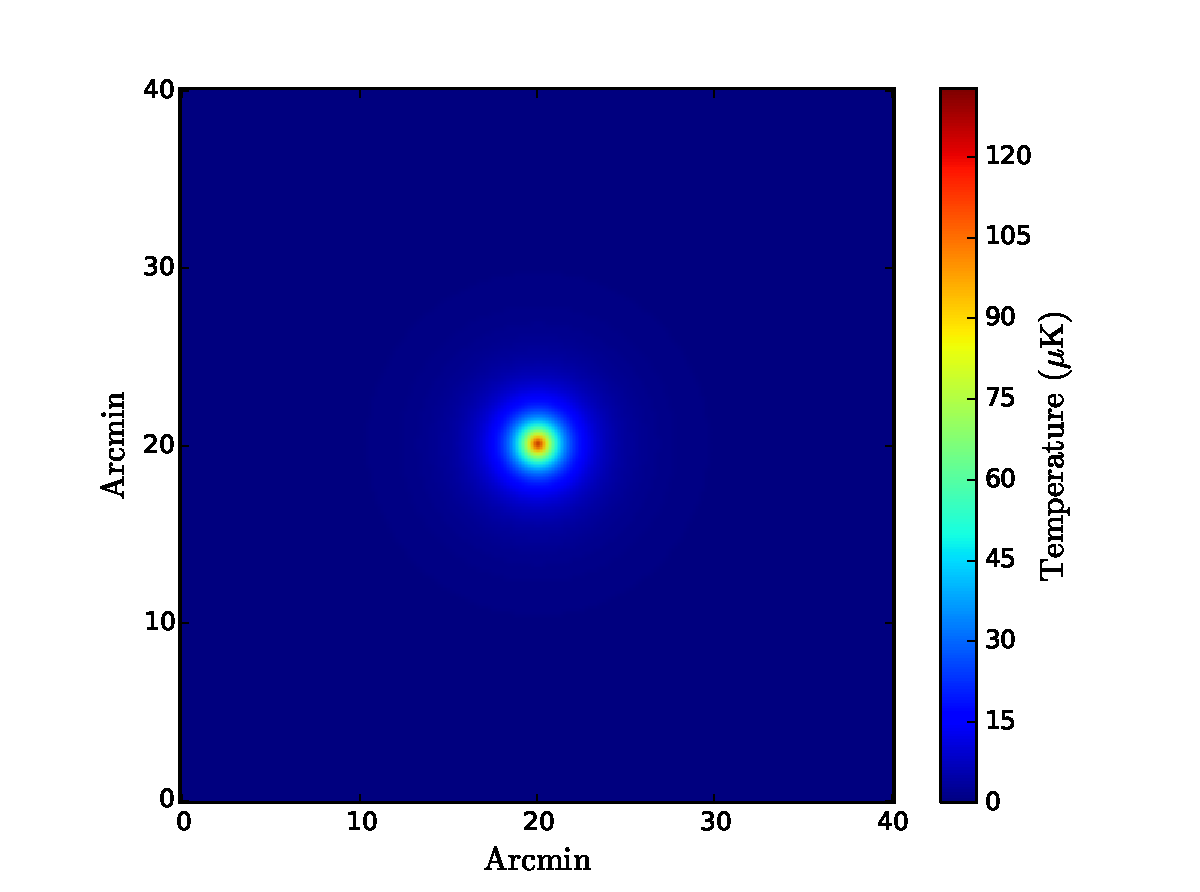
\includegraphics[scale=1.10, width=0.30\textwidth]{2.5_.22hm.pdf}
    }
    \hfill
    \subfloat[M = $3.5\times 10^{14} M_{\odot}$, Z= 0.22\label{subfig-2:dummy}]{%
      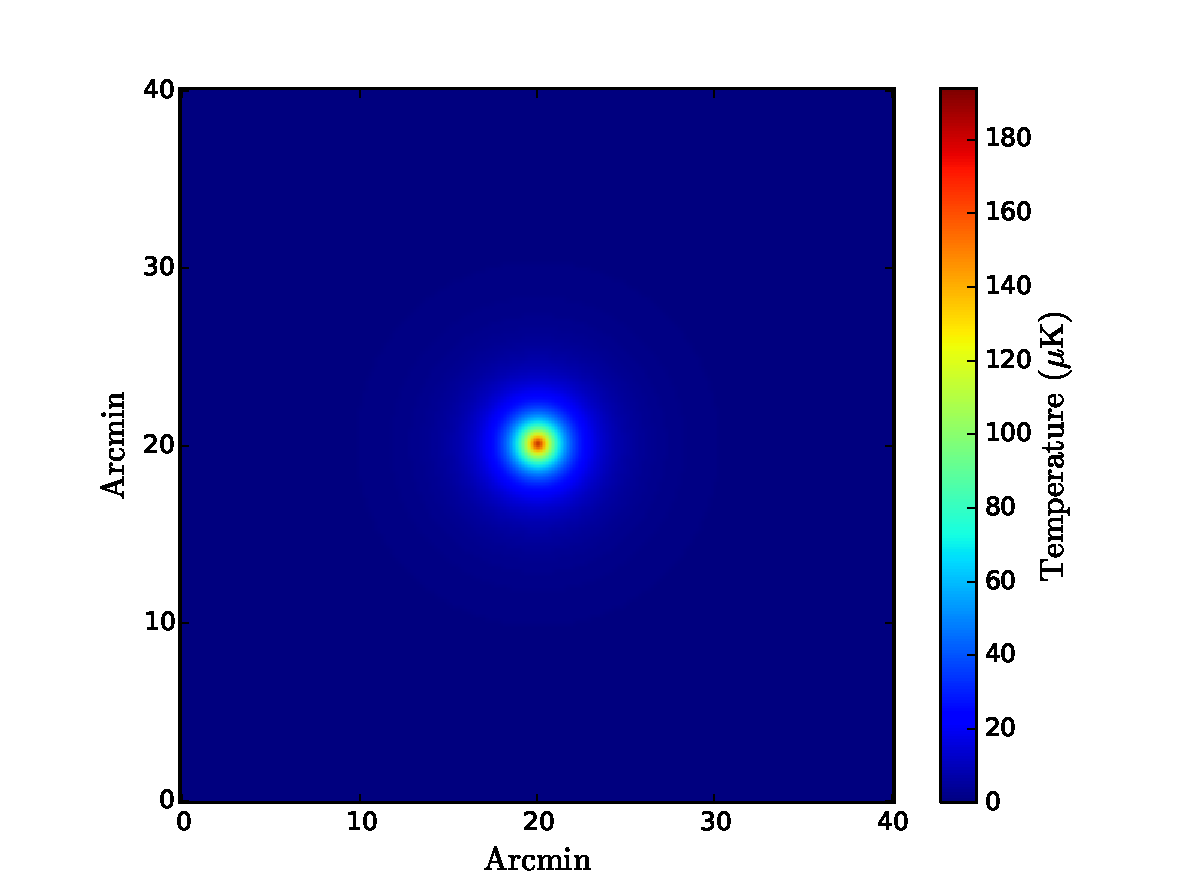
\includegraphics[scale=1.10, width=0.30\textwidth]{3.5_.22hm.pdf}
    }
    \hfill
    \subfloat[M = $4.5\times 10^{14} M_{\odot}$, Z= 0.22\label{subfig-2:dummy}]{%
      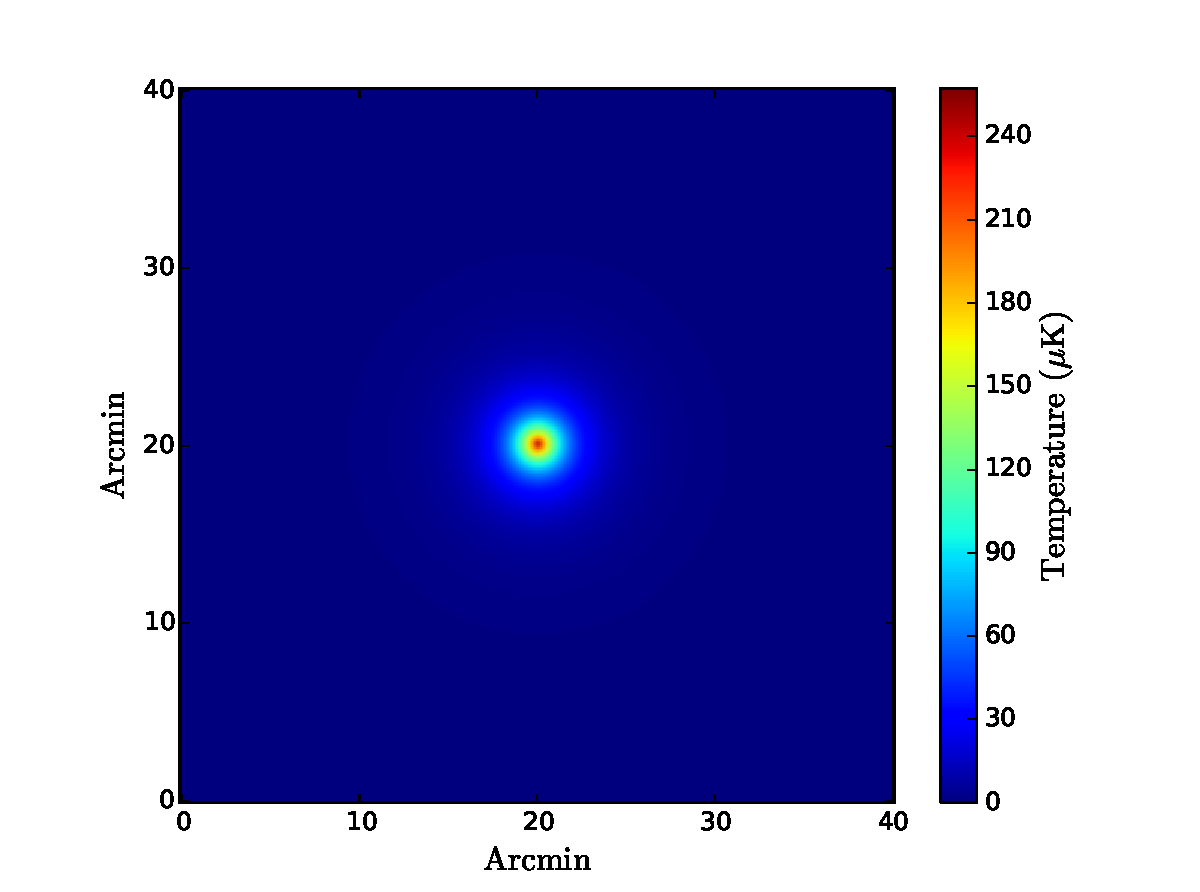
\includegraphics[scale=1.10, width=0.30\textwidth]{4.5_.22hm.pdf}
	}
    \vfill
    \subfloat[M = $2.5\times 10^{14} M_{\odot}$, Z= 0.55\label{subfig-2:dummy}]{%
      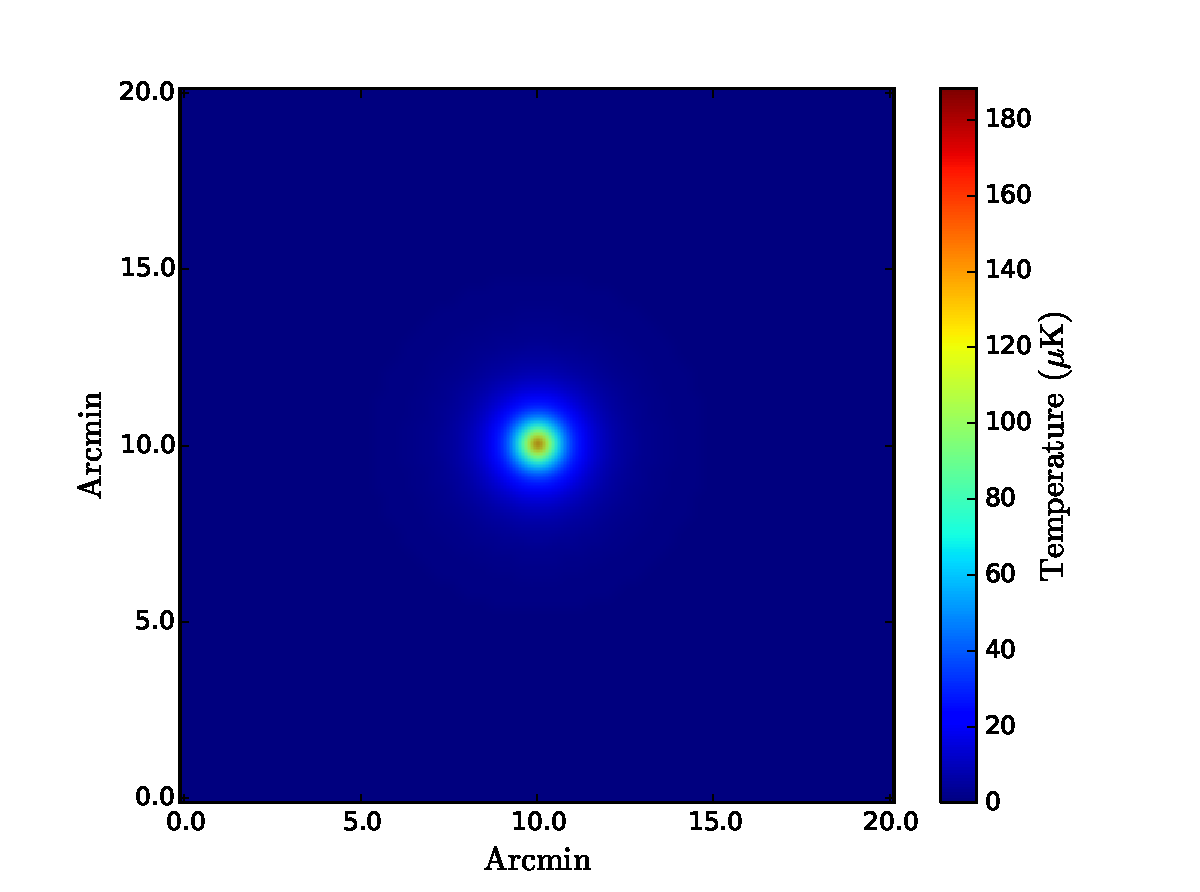
\includegraphics[scale=1.10, width=0.30\textwidth]{2.5_.55hm.pdf}
	}
    \hfill
    \subfloat[M = $3.5\times 10^{14} M_{\odot}$, Z= 0.55\label{subfig-2:dummy}]{%
      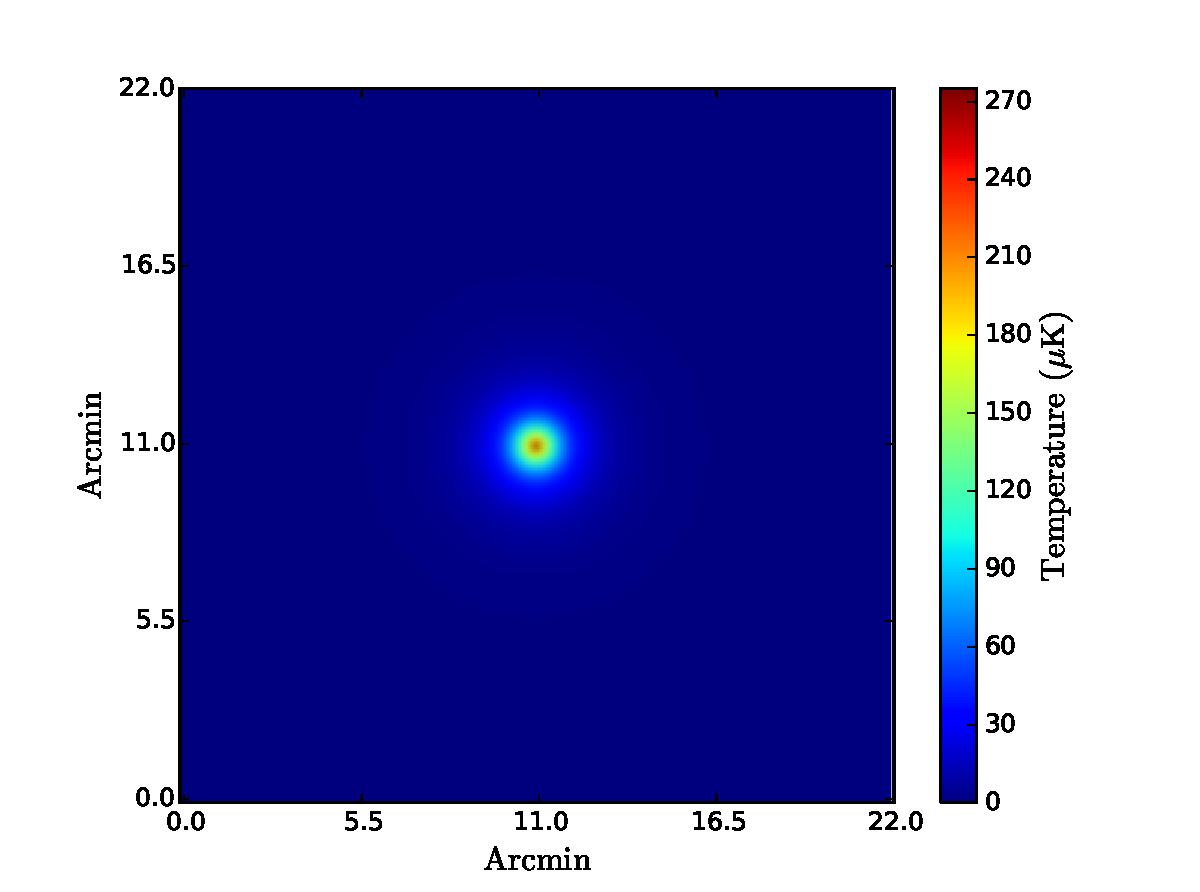
\includegraphics[scale=1.10, width=0.30\textwidth]{3.5_.55hm.pdf}
	}
    \hfill
    \subfloat[M = $4.5\times 10^{14} M_{\odot}$, Z= 0.55\label{subfig-2:dummy}]{%
      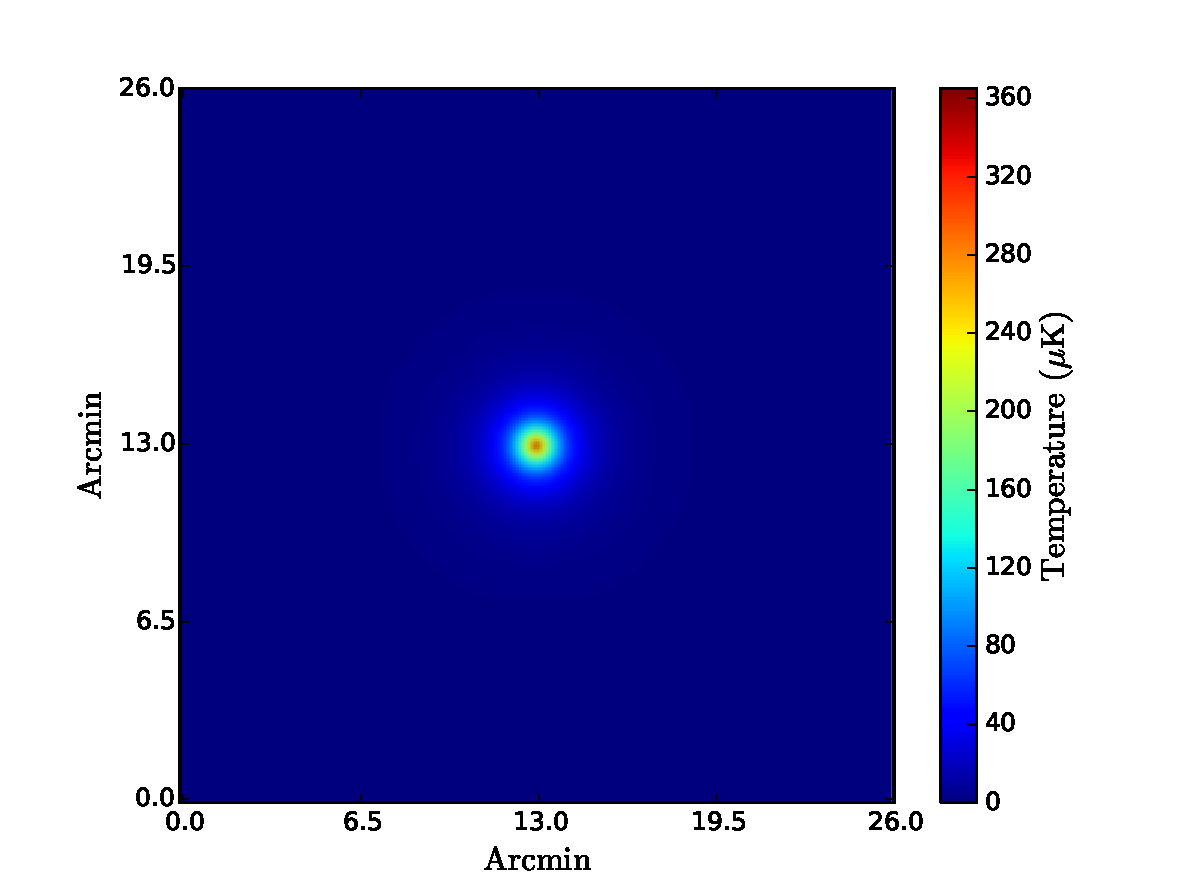
\includegraphics[scale=1.10, width=0.30\textwidth]{4.5_.55hm.pdf}
	}
    \vfill
    \subfloat[M = $2.5\times 10^{14} M_{\odot}$, Z= 1.00\label{subfig-2:dummy}]{%
      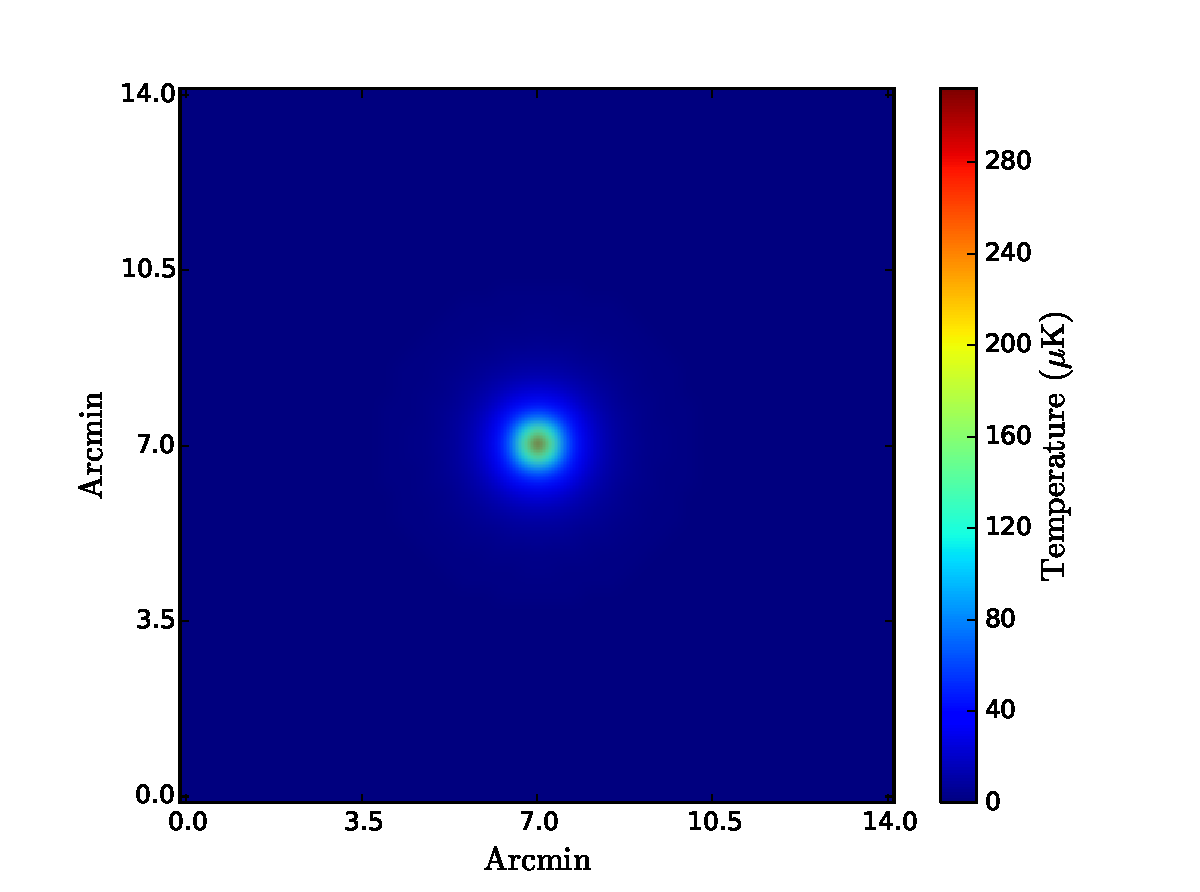
\includegraphics[scale=1.10, width=0.30\textwidth]{2.5_1hm.pdf}
	}
    \hfill
    \subfloat[M = $3.5\times 10^{14} M_{\odot}$, Z= 1.00\label{subfig-2:dummy}]{%
      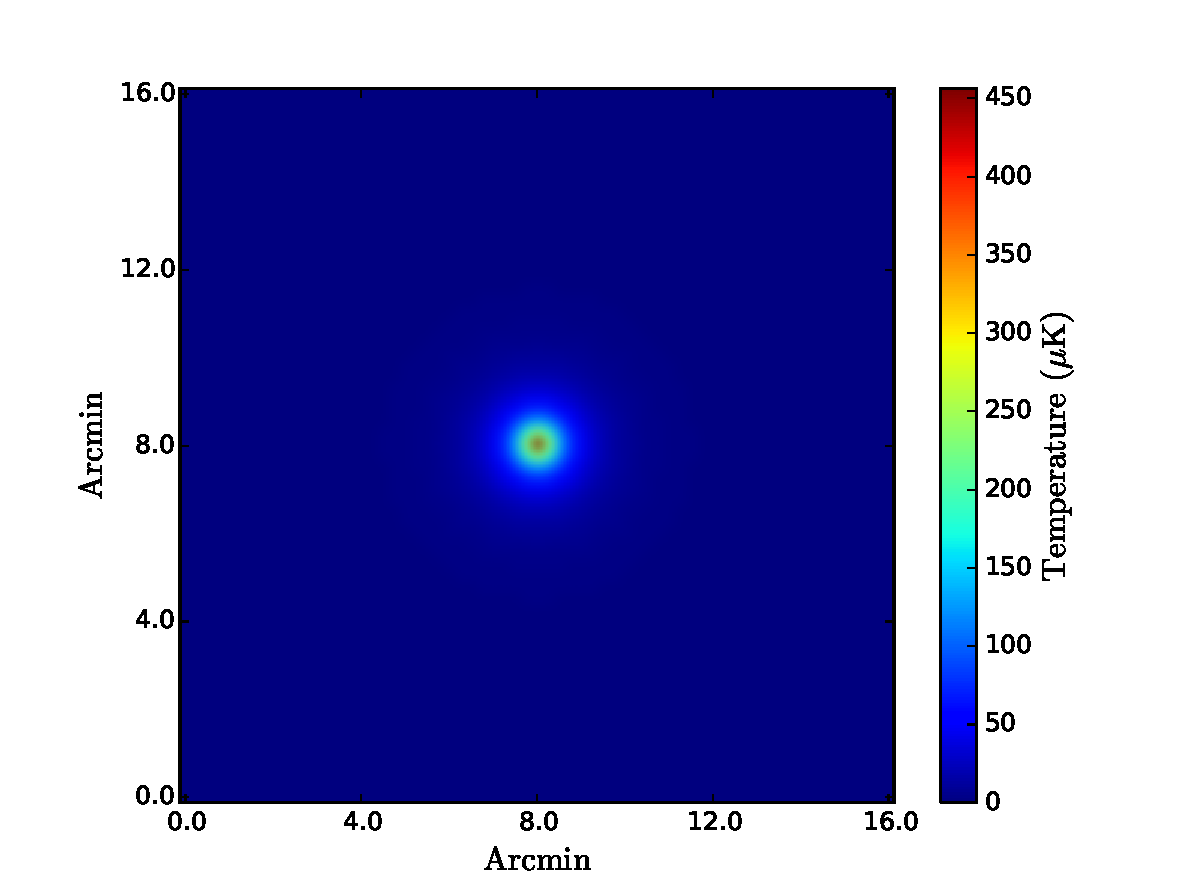
\includegraphics[scale=1.10, width=0.30\textwidth]{3.5_1hm.pdf}
	}
    \hfill
    \subfloat[M = $4.5\times 10^{14} M_{\odot}$, Z = 1.00\label{subfig-2:dummy}]{%
      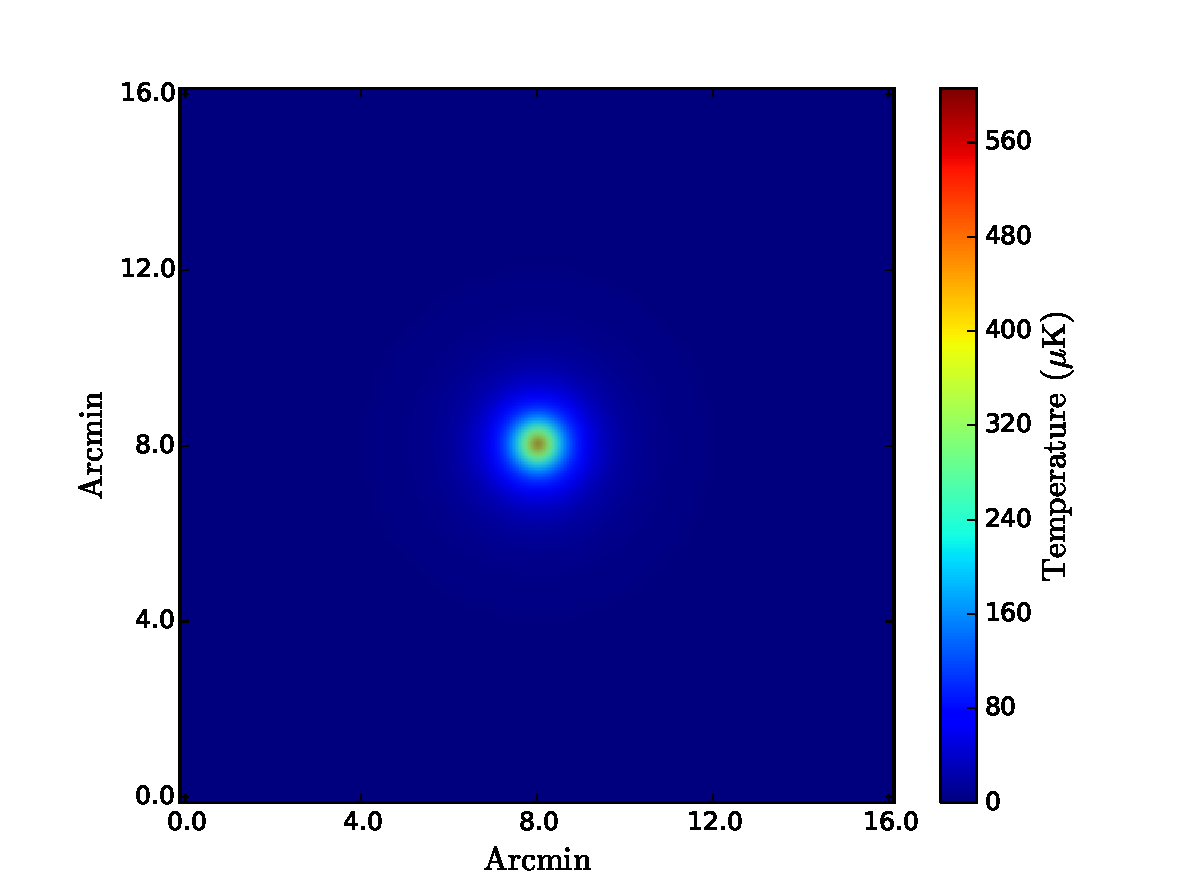
\includegraphics[scale=1.10, width=0.30\textwidth]{4.5_1hm.pdf}
	}
    \caption{Heat Maps Over Mass and Redshift Ranges}
    \label{fig:dummy}
  \end{figure}

Using these two dimensional heat maps, we created full sky maps. Each map was approxiamately 45 $deg^2$ and contained noise as well as clusters distributed at random locations on the map of the sky. The mass of the clusters were randomly drawn from a normal distribution around a mean value of $3.5\times 10^{14} M_{\odot}$ with a variance of $1.0\times 10^{14} M_{\odot}$. We take the absolute value when any negative mass value is selected, thus there is a double selction of lower mass clusters in the range of approxiamately $0.0\times 10^{14} M_{\odot}$ and $1.5\times 10^{14} M_{\odot}$. The redshift of the clusters were also randomly drawn from a flat distribution ranging over values of 0.2 to 1.2. The white noise contained in each sky map was normally distributed about a mean of zero, with a variance of 18.0 $\mu K$ - arcmin as suggested for the 150 GHz observing ban in Bleem (2009).  Once created a typical full sky map looks something like figure 5. Where we have produced two seperate realizations (same noise levels but different containing 25 clusters each. 

\begin{figure}[!ht]
    \subfloat[Realization 1\label{subfig-1:dummy}]{%
      \includegraphics[scale=1.10, width=.5\textwidth]{Full_Sky_Map.pdf}
    }
    \hfill
    \subfloat[Realization 2\label{subfig-2:dummy}]{%
      \includegraphics[scale=1.10, width=.5\textwidth]{Full_Sky_Map1.pdf}
    }
    \caption{Full Sky Realizations}
    \label{fig:dummy}
  \end{figure}

With this then we've described our process for creating the simulation. We then use these full sky maps to extract a resonable measure of the signal to noise ratio we can expect, specfically on the periphery of clusters. To do this we simply went in reverse, using our full sky maps to reconstruct an Arnaud profile and seeing how accurately our simulated results matched our expected results. We acheive this result by first cutting out smaller "postage" size cut outs of each cluster in a given full sky map. The size of this cut out is determined by the Arnaud profile of the cluster. Thus, for example, if the cluster has a mass of  $2.0\times 10^{14} M_{\odot}$ and a redshift of 0.4, then looking at the Arnaud profile we create a cut out which will encompass the entire approxiamately 14 arcmin radial range that cluster should encompass. We have reproduced a number of these cutouts as examples in figure 6, each plot is titled by its mass and redshift. 

\begin{figure}[!ht]
    \subfloat[M = $1.7\times 10^{14} M_{\odot}$, Z= 0.40\label{subfig-1:dummy}]{%
      \includegraphics[scale=1.10, width=0.30\textwidth]{Cutout21.pdf}
    }
    \hfill
    \subfloat[M = $3.6\times 10^{14} M_{\odot}$, Z= 0.50\label{subfig-2:dummy}]{%
      \includegraphics[scale=1.10, width=0.30\textwidth]{Cutout3.pdf}
    }
    \hfill
    \subfloat[M = $3.9\times 10^{14} M_{\odot}$, Z= 0.90\label{subfig-2:dummy}]{%
      \includegraphics[scale=1.10, width=0.30\textwidth]{Cutout6.pdf}
	}
    \vfill
    \subfloat[M = $3.5\times 10^{14} M_{\odot}$, Z= 1.00\label{subfig-2:dummy}]{%
      \includegraphics[scale=1.10, width=0.30\textwidth]{Cutout7.pdf}
	}
    \hfill
    \subfloat[M = $1.9\times 10^{14} M_{\odot}$, Z= 0.90\label{subfig-2:dummy}]{%
      \includegraphics[scale=1.10, width=0.30\textwidth]{Cutout9.pdf}
	}
    \hfill
    \subfloat[M = $3.1\times 10^{14} M_{\odot}$, Z= 1.00\label{subfig-2:dummy}]{%
      \includegraphics[scale=1.10, width=0.30\textwidth]{Cutout11.pdf}
	}
    \vfill
    \subfloat[M = $6.8\times 10^{14} M_{\odot}$, Z= 0.30\label{subfig-2:dummy}]{%
      \includegraphics[scale=1.10, width=0.30\textwidth]{Cutout13.pdf}
	}
    \hfill
    \subfloat[M = $5.0\times 10^{14} M_{\odot}$, Z= 0.80\label{subfig-2:dummy}]{%
      \includegraphics[scale=1.10, width=0.30\textwidth]{Cutout15.pdf}
	}
    \hfill
    \subfloat[M = $4.0\times 10^{14} M_{\odot}$, Z = 0.80\label{subfig-2:dummy}]{%
      \includegraphics[scale=1.10, width=0.30\textwidth]{Cutout17.pdf}
	}
    \caption{Simulated Heat Maps Over Various Masses and Redshifts}
    \label{fig:dummy}
  \end{figure}

We utilized two different binning strategies in creating Arnaud profiles from our two dimensional heat maps: (1.) We do an exact radial distance binning in which each quarter archmin size pixel of a specific radial distance from the center of the two dimensional heat map is averaged over. Thus if at 8.76 archmintues from the center we find 10 pixels we average over the temperature values we find in these 10 pixels and take this value to be the temperature at that radial distance. (2.) We bin in radial ranges, using this method we take all temperature values within a radial range, such as between 5.70 - 8.70 archmintes and average all of these values as well as averaging the radial distances in the radial range. We then take these averages to be the temperture and radial distance respectively. 

In figures 7 and 8  we have produced a number of sample plots in which we compare utilizing the first binning method verses using the second. In figure 7 we plot samples using the first binning method and in figure 8 we plot samples using the second binning method. The dots are the averaged temperature values at that specific radial distance, while the red line is the expected Arnaud profile given the mass and redshift of the cluster.  Once again each plot is labeled by its mass and redshift. 

\begin{figure}[!ht]
    \subfloat[M = $1.7\times 10^{14} M_{\odot}$, Z= 0.40\label{subfig-1:dummy}]{%
      \includegraphics[scale=1.10, width=0.30\textwidth]{Scatter21.pdf}
    }
    \hfill
    \subfloat[M = $3.6\times 10^{14} M_{\odot}$, Z= 0.50\label{subfig-2:dummy}]{%
      \includegraphics[scale=1.10, width=0.30\textwidth]{Scatter3.pdf}
    }
    \hfill
    \subfloat[M = $3.9\times 10^{14} M_{\odot}$, Z= 0.90\label{subfig-2:dummy}]{%
      \includegraphics[scale=1.10, width=0.30\textwidth]{Scatter6.pdf}
	}
    \caption{Selected Unbinned Simulated Arnaud Profiles Over Various Masses and Redshifts}
    \label{fig:dummy}
  \end{figure}

\begin{figure}[!ht]
    \subfloat[M = $1.7\times 10^{14} M_{\odot}$, Z= 0.40\label{subfig-1:dummy}]{%
      \includegraphics[scale=1.10, width=0.30\textwidth]{Bin_Scatter1.pdf}
    }
    \hfill
    \subfloat[M = $3.6\times 10^{14} M_{\odot}$, Z= 0.50\label{subfig-2:dummy}]{%
      \includegraphics[scale=1.10, width=0.30\textwidth]{Bin_Scatter3.pdf}
    }
    \hfill
    \subfloat[M = $3.9\times 10^{14} M_{\odot}$, Z= 0.90\label{subfig-2:dummy}]{%
      \includegraphics[scale=1.10, width=0.30\textwidth]{Bin_Scatter6.pdf}
	}
    \caption{Selected Binned Simulated Arnaud Profiles Over Various Masses and Redshifts}
    \label{fig:dummy}
  \end{figure}

We can then take these profiles, both the Arnaud and the two demisional heat maps and bin and stack them according to redshift and mass to perform our signal to noise ratio analysis. However, in order to simplify matters in the binning and stacking process, we used indentical clusters of mass $3.2\times 10^{14} M_{\odot}$ and redshift 0.5. Thus, in the anaylsis which follows when we refer to number of simulations performed we are refering to the number of noise realizations we used and when we refer to the number of clusters stacked we are refering to the number of clusters of mass $3.2\times 10^{14} M_{\odot}$ and redshift 0.5 that we stacked to obtain our measurment. Thus, if we say we performed 100 simulations with 25 stacked clusters each, we mean that we created 100 different full sky map realizations, each of which contained 25 clusters. For each full sky map realization we then stack the 25 clusters of equal mass and redshift contained in that particular fully sky map realization. 

 We performed three different types of signal to noise anaylsis using both of the two radial binning methods already explained.  We now breifly describe each of the three typse of measurments we performed in turn and present the results from each. 

The first method was an error anaylsis. We first produced 10, 25, 50, and 100 different full sky map realizations. On these full sky realizations we plotted at random locations for each realization, one cluster (of mass $3.2\times 10^{14} M_{\odot}$ and redshift 0.5 as noted before). We then took the average values between all of the realizations with a specific radial bin. So for example, say we produced 15 full sky map realizations. At some random point on each of the 15 maps one cluster was located.  Thus, in total we have 15 clusters. Each of these 15 clusters have a particular temperature value assoicated with a specific radial value. So for each radial distance we take the average temperature among the 15 clusters we have produced from the 15 different full sky realizations. We then compare these average temperature values to the expected temperature value that we dervive from the Arnaud profile of a cluster of mass $3.2\times 10^{14} M_{\odot}$ and redshift 0.5. We take the deviation of our averaged temperature values from the expected temperatures as given by the Arnaud Profile and plot these as our error bars, on the average temperatue values . We do this anaylsis for both binning methods. As expected as the number of realizations increases the mean error decreases according to:

We summarize the results of this anaylsis in figures 9 and 10. In figure 9 we utilize the first binning technique in which we do not average over data in mulitple different radial bins and in figure 10 we utilize the second binning technique in which we do average over data in mulitple radial bins:

\begin{figure}[!ht]
    \subfloat[5 Simulations\label{subfig-1:dummy}]{%
      \includegraphics[scale=0.50, width=.50\textwidth]{Mean_PercentError_5Sim_1Clust.pdf}
   	}
    \hfill
    \subfloat[25 Simulations\label{subfig-2:dummy}]{%
      \includegraphics[scale=0.50, width=.50\textwidth]{Mean_PercentError_25Sim_1Clust.pdf}
	}
    \hfill
    \subfloat[50 Simulations\label{subfig-2:dummy}]{%
      \includegraphics[scale=0.50, width=.50\textwidth]{Mean_PercentError_50Sim_1Clust.pdf}
	}
    \hfill
    \subfloat[100 Simulations\label{subfig-2:dummy}]{%
      \includegraphics[scale=0.50, width=.50\textwidth]{Mean_PercentError_100Sim_1Clust.pdf}
	}
    \caption{Unaveraged Binned Means}
    \label{}
  \end{figure}

\begin{figure}[!ht]
    \subfloat[5 Simulations\label{subfig-1:dummy}]{%
      \includegraphics[scale=0.50, width=.50\textwidth]{AVG_Mean_PercentError_5Sim_1Clust.pdf}
   	}
    \hfill
    \subfloat[25 Simulations\label{subfig-2:dummy}]{%
      \includegraphics[scale=0.50, width=.50\textwidth]{AVG_Mean_PercentError_25Sim_1Clust.pdf}
	}
    \hfill
    \subfloat[50 Simulations\label{subfig-2:dummy}]{%
      \includegraphics[scale=0.50, width=.50\textwidth]{AVG_Mean_PercentError_50Sim_1Clust.pdf}
	}
    \hfill
    \subfloat[100 Simulations\label{subfig-2:dummy}]{%
      \includegraphics[scale=0.50, width=.50\textwidth]{AVG_Mean_PercentError_100Sim_1Clust.pdf}
	}
    \caption{Averaged Binned Means}
    \label{}
  \end{figure}

Our second method of anaylsis measured the variation and standard deviation of the data. Again we produced 10, 25, 50, and 100 different full sky map realization batches and on each of these realizations plotted at random locations, one cluster of mass $3.2\times 10^{14} M_{\odot}$ and redshift 0.5. However, this time we created two different types of plots: (1.) The mean value within a given radial bin divided by the variance of the values within that given radial bin as a function of radial distance and (2.) The variance of the values within a given radial bin as a function of radial distance. Naturally, the latter plot was displayed a flat distribution, that is to say that the variance was generally about the same at all radial distances and the average of the variance was constant as a function of number of realizations used (e.g. 10, 25, 50 and 100 realizations). This is expected since the only variance introduced into the full sky maps is due to the gaussian white noise present in the realizations. However, the former plots, of mean values over the variance as a function of radial distance were not flat, instead we observe anexponetionally declining function. This however, is most likely less due to any net movement in the variance and more due to the natural decline in the mean of the temperature in each radial bin. We display our results of the mean over variance plots in figures 11 and 12. Similiar to figures 9 and 10, in figure 11 we utilize the first binning technique in which we do not average over data in mulitple different radial bins and in figure 12 we utilize the second binning technique in which we do average over data in mulitple radial bins:

\begin{figure}[!ht]
    \subfloat[5 Simulations\label{subfig-1:dummy}]{%
      \includegraphics[scale=0.50, width=.50\textwidth]{Mean_Var_5Sim_1Clust.pdf}
   	}
    \hfill
    \subfloat[25 Simulations\label{subfig-2:dummy}]{%
      \includegraphics[scale=0.50, width=.50\textwidth]{Mean_Var_25Sim_1Clust.pdf}
	}
    \hfill
    \subfloat[50 Simulations\label{subfig-2:dummy}]{%
      \includegraphics[scale=0.50, width=.50\textwidth]{Mean_Var_50Sim_1Clust.pdf}
	}
    \hfill
    \subfloat[100 Simulations\label{subfig-2:dummy}]{%
      \includegraphics[scale=0.50, width=.50\textwidth]{Mean_Var_100Sim_1Clust.pdf}
	}
    \caption{Unaveraged Binned Means}
    \label{}
  \end{figure}

\begin{figure}[!ht]
    \subfloat[5 Simulations\label{subfig-1:dummy}]{%
      \includegraphics[scale=0.50, width=.50\textwidth]{AVG_Mean_Var_5Sim_1Clust.pdf}
   	}
    \hfill
    \subfloat[25 Simulations\label{subfig-2:dummy}]{%
      \includegraphics[scale=0.50, width=.50\textwidth]{AVG_Mean_Var_25Sim_1Clust.pdf}
	}
    %\hfill
    %\subfloat[50 Simulations\label{subfig-2:dummy}]{%
      %\includegraphics[scale=0.50, width=.50\textwidth]{AVG_Mean_Var_50Sim_1Clust.pdf}
	%}
    %\hfill
    %\subfloat[100 Simulations\label{subfig-2:dummy}]{%
      %\includegraphics[scale=0.50, width=.50\textwidth]{AVG_Mean_Var_100Sim_1Clust.pdf}
	%}
    \caption{Averaged Binned Means}
    \label{}
  \end{figure}

Our third analysis was to measure the percentage of our measurement which was noise as a function of radial distance. We accomplished this by borrowing much of the apparatus of the first two methods of anaylsis but 

\section{Discussion}

\end{document}
